% ===========================================================================
% MODELO DE RELATORIO  ·  ENE0046 Laboratorio de Eletronica  ·  2026/2
%
% Como usar
%   1. Preencha o bloco IDENTIFICACAO logo abaixo.
%   2. Deixe comentados os autores que nao existirem. Um autor fica centralizado,
%      dois dividem a linha, tres ocupam tercos.
%   3. Substitua o texto de cada secao pelo seu. As orientacoes que estao la
%      dizem o que se espera em cada uma.
%   4. Compile com pdflatex duas vezes, ou com latexmk -pdf.
%
% Estrutura
%   Roteiro 1 nao tem bancada: use so a subsecao 4.1 e a 5.1, e compare o calculo
%   analitico com a simulacao de projeto.
%   Roteiros 2 a 7 usam a estrutura inteira.
%
% O arquivo estilo-relatorio.tex e a imagem logo-unb.png devem estar na mesma
% pasta deste arquivo.
% ===========================================================================
\documentclass[11pt,a4paper]{article}
% !TeX root = modelo-relatorio.tex
% Formatacao do relatorio. Compile o modelo-relatorio.tex, nao este arquivo.
\usepackage[T1]{fontenc}
\usepackage[utf8]{inputenc}
\usepackage[brazil]{babel}
\usepackage[a4paper,top=1.6cm,bottom=1.8cm,left=2.1cm,right=2.1cm]{geometry}
\usepackage[default]{lato}
\usepackage{amsmath,amssymb}
\usepackage{siunitx}
\usepackage{graphicx}
\usepackage{booktabs,array,longtable,colortbl}
\usepackage{enumitem}
\usepackage{tcolorbox}
\usepackage{xcolor}
\usepackage{tikz}
\usepackage{titlesec}
\usepackage{fancyhdr}
\usepackage{caption}
\usepackage{etoolbox}
\usepackage{placeins}
\usepackage{float}
\usepackage[colorlinks=true,linkcolor=azul,urlcolor=azul,citecolor=azul]{hyperref}
\tcbuselibrary{skins,breakable}

\definecolor{azul}{HTML}{0A4B8C}
\definecolor{azulclaro}{HTML}{E8F0F8}
\definecolor{verde}{HTML}{0B7A4B}
\definecolor{cinza}{HTML}{5B6672}
\definecolor{cinzaclaro}{HTML}{F4F6F8}
\definecolor{vinho}{HTML}{B04A4A}
\definecolor{vinhoclaro}{HTML}{FBF2F2}

\sisetup{output-decimal-marker={,}, per-mode=symbol}
\setlength{\parindent}{0pt}
\setlength{\parskip}{6pt plus 1pt}
\setlist{itemsep=3pt, topsep=4pt, parsep=0pt, leftmargin=1.3em}
\renewcommand{\arraystretch}{1.25}
\linespread{1.06}

% ---- secoes numeradas com marcador colorido -------------------------------
\titleformat{\section}[hang]
  {\Large\bfseries\color{azul}}
  {\raisebox{-1pt}{\tikz\node[fill=azul,text=white,rounded corners=2pt,
     inner sep=3pt,minimum width=20pt,align=center]{\bfseries\thesection};}}
  {10pt}{}
\titlespacing*{\section}{0pt}{16pt plus 3pt}{6pt}
\titleformat{\subsection}{\large\bfseries\color{cinza}}{\thesubsection}{8pt}{}
\titlespacing*{\subsection}{0pt}{11pt plus 2pt}{3pt}

% ---- legendas -------------------------------------------------------------
\captionsetup{font=small,labelfont={bf,color=azul},labelsep=period,skip=6pt}

% ---- identificacao --------------------------------------------------------
\newcommand{\autorA}{}\newcommand{\matA}{}
\newcommand{\autorB}{}\newcommand{\matB}{}
\newcommand{\autorC}{}\newcommand{\matC}{}
\newcommand{\autorum}[2]{\renewcommand{\autorA}{#1}\renewcommand{\matA}{#2}}
\newcommand{\autordois}[2]{\renewcommand{\autorB}{#1}\renewcommand{\matB}{#2}}
\newcommand{\autortres}[2]{\renewcommand{\autorC}{#1}\renewcommand{\matC}{#2}}

\newcommand{\disciplina}{CIC0236 · Teleinformática e Redes 2}
\newcommand{\semestre}{2026/2}
\newcommand{\turma}{}
\newcommand{\roteironum}{}
\newcommand{\roteirotema}{}
\newcommand{\aturma}[1]{\renewcommand{\turma}{#1}}
\newcommand{\roteiro}[2]{\renewcommand{\roteironum}{#1}\renewcommand{\roteirotema}{#2}}

\newcommand{\umautor}[2]{%
  \begin{minipage}[t]{\dimexpr\linewidth-4pt\relax}\centering
    \parbox[t][30pt][t]{\linewidth}{\centering
      {\fontsize{10.5}{12.5}\selectfont #1}}\\[-2pt]
    {\color{cinza}\fontsize{9}{11}\selectfont\texttt{#2}}
  \end{minipage}}

\newcounter{nautores}
\newcommand{\blocoautores}{%
  \setcounter{nautores}{0}%
  \ifdefempty{\autorA}{}{\stepcounter{nautores}}%
  \ifdefempty{\autorB}{}{\stepcounter{nautores}}%
  \ifdefempty{\autorC}{}{\stepcounter{nautores}}%
  \ifnum\value{nautores}=0
    \begin{center}\color{vinho}\bfseries
      Preencha ao menos um autor no preâmbulo do arquivo.
    \end{center}
  \else
    \begin{center}
    \ifcase\value{nautores}\or
      % --- um autor: ocupa o centro
      \begin{minipage}{0.5\textwidth}\umautor{\autorA}{\matA}\end{minipage}%
    \or
      % --- dois autores: metades
      \begin{minipage}{0.42\textwidth}\umautor{\autorA}{\matA}\end{minipage}\hspace{0.04\textwidth}%
      \begin{minipage}{0.42\textwidth}\umautor{\autorB}{\matB}\end{minipage}%
    \or
      % --- tres autores: tercos
      \begin{minipage}{0.31\textwidth}\umautor{\autorA}{\matA}\end{minipage}\hspace{0.015\textwidth}%
      \begin{minipage}{0.31\textwidth}\umautor{\autorB}{\matB}\end{minipage}\hspace{0.015\textwidth}%
      \begin{minipage}{0.31\textwidth}\umautor{\autorC}{\matC}\end{minipage}%
    \fi
    \end{center}
  \fi}

% ---- cabecalho do relatorio -----------------------------------------------
\newcommand{\capa}{%
\begin{tcolorbox}[colback=azul,colframe=azul,boxrule=0pt,arc=4pt,
  left=16pt,right=16pt,top=13pt,bottom=13pt]
\color{white}
\begin{minipage}{0.76\textwidth}
  {\fontsize{9}{11}\selectfont\textbf{\MakeUppercase{\disciplina{} · \semestre{}}}}\\[6pt]
  {\fontsize{22}{25}\selectfont\bfseries Relatório da Entrega \roteironum}\\[3pt]
  {\fontsize{12.5}{15}\selectfont \roteirotema}
\end{minipage}\hfill
\begin{minipage}{0.2\textwidth}\raggedleft
  \colorbox{white}{\hspace{2pt}\raisebox{-2pt}{
\includegraphics[height=30pt]{logo-unb.png}}\hspace{2pt}}
\end{minipage}
\end{tcolorbox}
\vspace{10pt}
\blocoautores
\ifdefempty{\turma}{}{%
  \begin{center}{\color{cinza}\fontsize{9}{11}\selectfont Turma \turma}\end{center}}
\vspace{4pt}
{\color{azulclaro}\hrule height 2pt}
\vspace{2pt}}

% ---- caixas auxiliares ----------------------------------------------------
\newtcolorbox{formula}{colback=azulclaro,colframe=azul,boxrule=0.8pt,arc=3pt,
  left=12pt,right=12pt,top=9pt,bottom=9pt}
\newtcolorbox{nota}[1]{colback=cinzaclaro,colframe=cinza,boxrule=0.8pt,arc=3pt,
  left=10pt,right=10pt,top=7pt,bottom=7pt,
  title={\textbf{#1}},fonttitle=\small\bfseries,coltitle=white,colbacktitle=cinza}
\newenvironment{resumo}
  {\vspace{6pt}\begin{center}\begin{minipage}{0.92\textwidth}
   \begin{tcolorbox}[colback=cinzaclaro,colframe=cinzaclaro,boxrule=0pt,arc=3pt,
     left=14pt,right=14pt,top=10pt,bottom=10pt,
     borderline west={2.5pt}{0pt}{azul}]
   {\color{azul}\fontsize{8}{10}\selectfont\textbf{RESUMO}}\\[4pt]
   \small}
  {\end{tcolorbox}\end{minipage}\end{center}\vspace{2pt}}

\newtcolorbox{espec}{colback=azulclaro,colframe=azul,boxrule=0.8pt,arc=3pt,
  left=12pt,right=12pt,top=9pt,bottom=9pt,
  title={\textbf{Especificação da matrícula}},fonttitle=\bfseries,
  coltitle=white,colbacktitle=azul}

% ---- rodape ---------------------------------------------------------------
\pagestyle{fancy}\fancyhf{}
\renewcommand{\headrulewidth}{0pt}
\renewcommand{\footrulewidth}{0.4pt}
\fancyfoot[L]{\color{cinza}\fontsize{8}{10}\selectfont \disciplina{} · \semestre{} · Entrega \roteironum}
\fancyfoot[R]{\color{cinza}\fontsize{8}{10}\selectfont \thepage}

\newlist{referencias}{itemize}{1}
\setlist[referencias]{label={}, leftmargin=1.1em, itemindent=-1.1em,
                     itemsep=3pt, topsep=2pt, parsep=0pt}

\newcommand{\mat}[1]{\texttt{\textbf{#1}}}


% --------------------------- IDENTIFICACAO ---------------------------------
\roteiro{1}{Stop-and-Wait (SAW)}
\aturma{01}

\autorum{Enzo Morrone de Azevedo Muniz}{221035442}
\autordois{Luca Valderramos Cirino}{211066140}
\autortres{Raul Myron Silva Amorim}{200049712}
% ---------------------------------------------------------------------------

\begin{document}
\capa

\begin{resumo}
Escreva este parágrafo por último, com 100 a 150 palavras. Diga o que você projetou, sob
qual especificação, o que simulou ou mediu, o principal resultado numérico e a que
conclusão chegou. Quem ler só este parágrafo deve saber o que você fez e o que encontrou.
\end{resumo}

\section{Introdução}

Com a expanção da internet para além dos PCs, se tornou necessário desenvolver aplicações com tempo de resposta mínimo.
Isso deve-se ao celular, hoje o principal meio de se conectar na internet, que exige protocolos rápidos - devido as exigências dos usuários -
e confiáveis - devido a perda de pacotes esperada das comunicações sem fio.

Dessa forma, um pode pensar que o protocolo TCP é ideal, porém, devido a perda de pacotes, o mecanismo de confirmar pacotes com ACK
pode cause retransimições excessivas, diminuindo a largura de banda da comunicação. Já o UDP também não é ideal, visto que não garante
a comunicação confiável, apesar de permitir uma largura de banda melhor.

Assim, este relatório é parte 1 de 3, visando criar um novo protocolo que mistura os pontos fortes do UDP e TCP afim de obter
o melhor dos dois mundos - confiável e rápido. Neste relatório 1, usando o UDP como base, é implementado uma forma básica de 
comunicação confiável chamada \textit{Stop-and-Wait (SAW)}.

No \textit{Stop-and-Wait}, aquele que envia os pacotes, envia apenas um de cada vez, seguindo para o próximo apenas após receber um ACK.
Caso ocorra um timeout, o pacote é retransmitido até que se receba o respectivo ACK. Devido ao fato de que a maior parte do tempo é 
gasta esperando um ACK, o SAW não possui largura de banda boa, mas é uma forma fácil de implmentar comunicação confiável.

Este relatório está dividido em 3 secções principais: na implementação é dito como foi feito o código que implementa o protocolo;
nos resultados, tem-se a verificação da confiábilidade e dados de throughput e RTT da transimição; e por último na análise, os dados
dos resultados são comentádos.

\section{Implementação}

%%%%%%%%%%%%%%%%%%%%%%%%%%%%%%%%%%%%%%%%%%%%%%%%%%%%%%%%%%%%%%%%%%%%%%%%%%%%%%%%
colocar Fluxograma ou máquina de estados do cliente implementado
%%%%%%%%%%%%%%%%%%%%%%%%%%%%%%%%%%%%%%%%%%%%%%%%%%%%%%%%%%%%%%%%%%%%%%%%%%%%%%%%

\section{Resultados}

%%%%%%%%%%%%%%%%%%%%%%%%%%%%%%%%%%%%%%%%%%%%%%%%%%%%%%%%%%%%%%%%%%%%%%%%%%%%%%%%
colocar Checksum MD5 do arquivo recebido para cada um dos três testes — é a confirmação de que o cliente rodou de verdade
%%%%%%%%%%%%%%%%%%%%%%%%%%%%%%%%%%%%%%%%%%%%%%%%%%%%%%%%%%%%%%%%%%%%%%%%%%%%%%%%

%%%%%%%%%%%%%%%%%%%%%%%%%%%%%%%%%%%%%%%%%%%%%%%%%%%%%%%%%%%%%%%%%%%%%%%%%%%%%%%%
colocar Gráfico de throughput e RTT por segmento para pelo menos um dos arquivos
%%%%%%%%%%%%%%%%%%%%%%%%%%%%%%%%%%%%%%%%%%%%%%%%%%%%%%%%%%%%%%%%%%%%%%%%%%%%%%%%

\begin{figure}[H]
\centering
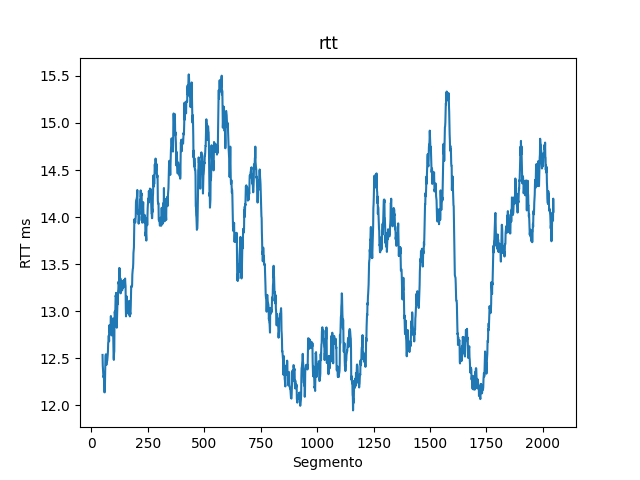
\includegraphics[width=0.8\linewidth]{grafico_rtt_small.png}
	\caption{Gráfico de RTT em millisegundos. Para melhor visualazação, está exibido uma média móvel simples de tamanho 50 dos valores reais.}
\label{fig:exemplo}
\end{figure}

\begin{figure}[H]
\centering
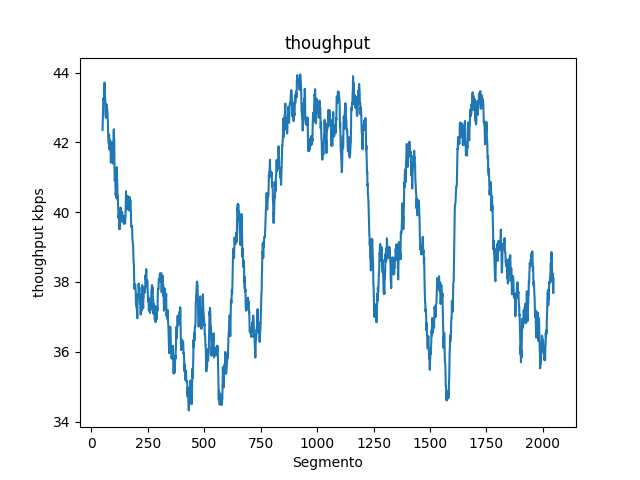
\includegraphics[width=0.8\linewidth]{grafico_thoughput_small.png}
\caption{Gráfico de throughput em kilobytes/segundo. Para melhor visualazação, está exibido uma média móvel simples de tamanho 50 dos valores reais.}
\label{fig:exemplo}
\end{figure}

%%%%%%%%%%%%%%%%%%%%%%%%%%%%%%%%%%%%%%%%%%%%%%%%%%%%%%%%%%%%%%%%%%%%%%%%%%%%%%%%
colocar Tabela comparativa entre throughput teórico e medido para os três arquivos (small, medium, large)
%%%%%%%%%%%%%%%%%%%%%%%%%%%%%%%%%%%%%%%%%%%%%%%%%%%%%%%%%%%%%%%%%%%%%%%%%%%%%%%%

\section{Analise}

%%%%%%%%%%%%%%%%%%%%%%%%%%%%%%%%%%%%%%%%%%%%%%%%%%%%%%%%%%%%%%%%%%%%%%%%%%%%%%%%
colocar:
Análise obrigatória no relatório:

a) Por que o throughput do SAW é limitado pelo RTT? Explique com suas palavras, usando os dados coletados como evidência.

b) Calcule o throughput teórico máximo usando a fórmula abaixo e compare com o throughput médio medido para cada arquivo:

$Throughput_{max} = (segment\_size × 8) / RTT_{medio}$
%%%%%%%%%%%%%%%%%%%%%%%%%%%%%%%%%%%%%%%%%%%%%%%%%%%%%%%%%%%%%%%%%%%%%%%%%%%%%%%%

%%%%%%%%%%%%%%%%%%%%%%%%%%%%%%%%%%%%%%%%%%%%%%%%%%%%%%%%%%%%%%%%%%%%%%%%%%%%%%%%
comandos latex para figura, tabela e essas caixas

\begin{figure}[H]
\centering
% \includegraphics[width=0.8\linewidth]{arquivo.png}
\fbox{\parbox[c][3.2cm][c]{0.8\linewidth}{\centering\color{cinza}
  substitua por \texttt{\textbackslash includegraphics}}}
\caption{Legenda descritiva. Diga o que a figura mostra e o que nela é relevante, e não
apenas o nome do circuito.}
\label{fig:exemplo}
\end{figure}

\begin{center}
\begin{tabular}{@{}lrrrr@{}}
\toprule
\textbf{Grandeza} & \textbf{Projeto} & \textbf{Sim. montagem} & \textbf{Medido} &
\textbf{Erro} \\
\midrule
& & & & \\
\bottomrule
\end{tabular}
\end{center}

\begin{nota}{Três comparações, três causas diferentes}

\smallskip
\textbf{Cálculo analítico contra simulação de projeto.} A conta está certa? Se aqui houver
diferença, procure na álgebra ou no esquemático.

\smallskip
\textbf{Simulação de projeto contra simulação da montagem.} Quanto custou a tolerância dos
componentes? A diferença aqui é a distância entre o valor nominal e o valor real da peça
que vocês pegaram.

\smallskip
\textbf{Simulação da montagem contra medição.} O modelo descreve o circuito real? Diferença
aqui aponta algo que o modelo não representa, como a resistência série do indutor, a
impedância da ponta de prova ou a banda do instrumento.
\end{nota}

\begin{espec}{azul}

\smallskip
\textbf{Cálculo analítico contra simulação de projeto.} A conta está certa? Se aqui houver
diferença, procure na álgebra ou no esquemático.

\end{espec}

\section{Conclusão}

Retome o objetivo que vocês anunciaram na introdução e responda se ele foi atingido,
apoiando a resposta em um número. Aponte a principal limitação do que foi feito e o que
ela impede de afirmar. Evite trazer resultado novo nesta seção.

\section{Referências}

\begin{referencias}
\item James F. Kurose \& Keith W. Ross, \emph{Redes de Computadores e a Internet - Uma nova Abordagem}, 8a Edição, Pearson Education / Makron Books.

\item Andrew S. Tanenbaum, \emph{Redes de Computadores}, Pearson Universidades, 5a Edição, 2011
\end{referencias}

\end{document}
